% Research proposal for the GDRFA Dubai Scientific Research Award (2nd cycle, deadline 15 Oct 2026).
% Build: bash build.sh  (pdflatex + bibtex, IEEEtran bibliography style). Same form as the other notes in this folder.
\documentclass[11pt,a4paper]{article}

\usepackage[margin=3cm]{geometry}
\usepackage[utf8]{inputenc}
\usepackage[T1]{fontenc}
\usepackage{amsmath,amssymb,amsthm}
\usepackage{microtype}
\usepackage{booktabs}
\usepackage{graphicx}
\usepackage{array}
\usepackage{enumitem}
\usepackage{cite}
\usepackage[dvipsnames]{xcolor}
\usepackage{tcolorbox}
\usepackage{tikz}
\usetikzlibrary{arrows.meta,positioning,calc,shapes.misc,fit,backgrounds}
\usepackage{pgfgantt}
\usepackage{caption}
\usepackage{subcaption}
\usepackage{placeins}
\usepackage{float}
\usepackage{rotating}
\usepackage{pdflscape}
\usepackage{afterpage}
\newcolumntype{L}[1]{>{\raggedright\arraybackslash}p{#1}}
\usepackage{xurl}
\usepackage[hidelinks]{hyperref}

\linespread{1.1}
\setlength{\parskip}{0.35em}
\setlist{itemsep=0.35em, topsep=0.4em}
\allowdisplaybreaks
\captionsetup{font=small,labelfont=bf}
\renewcommand{\floatpagefraction}{0.85}
\renewcommand{\topfraction}{0.9}
\renewcommand{\textfraction}{0.08}

\newtcolorbox{keybox}{colback=white, colframe=NavyBlue!55, boxrule=0.5pt, arc=0pt,
  left=10pt, right=10pt, top=6pt, bottom=6pt, before skip=12pt, after skip=12pt}

\definecolor{ink}{RGB}{30,30,30}
\definecolor{line1}{RGB}{70,110,160}
\definecolor{line2}{RGB}{170,70,50}
\definecolor{soft}{RGB}{235,238,243}
\definecolor{soft2}{RGB}{247,240,236}

\title{Refer or Clear\\[6pt]
\large Reference-conditioned detection of altered travel documents on designs never seen:\\ a public measurement for the first line\\[4pt] \normalsize Research proposal, GDRFA Dubai Scientific Research Award, second cycle}
\author{Hamza Abushahla and Mohamed I. AlHajri\\ \small American University of Sharjah}
\date{8 October 2026}

\begin{document}
\maketitle

\begin{abstract}
\noindent Dubai's border checks travel documents in two lines. About 1,600 first-line passport officers see every document for a few seconds and refer anything suspicious to a Document Examination Centre of about 50 experts. The centre's own figures for 2025 and the first half of 2026 are 20,307 referred examinations and 902 confirmed irregularities, a hit rate of 4.4 percent, and its head has said that paper forgeries are the easy part while electronically altered documents are the hard one. The first line already runs a commercial reader with a template library covering more than 80 countries. What no operator can measure, because no vendor publishes it, is how such a system behaves on a document design outside its library. Published research detectors do not help: they are single-image classifiers that score near 100 percent on designs they were trained on and fall to chance on designs they were not. We propose the learned form of what the reader already does by rule: a detector that receives the presented data page together with a clean reference of the same design and scores the deviation between them, so that the design becomes an input rather than something to memorize. We build the first paired, design-referenced forgery dataset from public sources, benchmark single-image and reference-conditioned detectors on identical samples under two protocols, unseen design within a dataset and unseen design across dataset, generator, capture and script, including an Arabic-script design, and report the result as a first-line referral rate at a fixed miss budget against the centre's published base rate. The architecture is built on a published change-detection framework with a difference-fusion variant and an attention-fusion variant, evaluated over a grid of backbones and transfer regimes. The deliverable to GDRFA is the measurement its vendor does not provide and the open dataset and protocol to repeat it on its own template library without any document leaving the centre.
\end{abstract}

\section{Introduction}
\label{sec:problem}

\paragraph{Two lines, and the hard cases sit on the first.} Every traveller's document at Dubai's ports is checked first by a passport officer at a counter, a smart-gate bank or, since September 2026, on a Click \& Travel handheld that reads the e-passport chip and matches the face in 12 to 15 seconds \cite{gdrfa2026clickandtravel,thenational2026click}. Anything the officer doubts goes to the second line, GDRFA's Document Examination Centre at Terminal 1, a forensic laboratory accredited to ISO/IEC 17025 with a passport reference database from more than 80 countries, a partnership with the German Federal Police document laboratory, and roughly 50 examiners \cite{gulfnews2026forgery,gulftoday2026forgery,uaejournal2025fake}. The three-tier structure the centre describes, about 1,600 first-line officers, a second line, and the centre itself, is the primary and secondary examination model of ICAO Doc 9303 \cite{icao9303p2,uaejournal2025fake}. The first line is where time is shortest. Frontex and INTERPOL describe their Quick Check Cards as a decision aid for front-line officers who ``have only seconds'' \cite{frontex2023quickcheck}.

\paragraph{The centre's own numbers.} Between January 2025 and June 2026 the centre conducted 20,307 technical examinations of travel documents and found 902 irregularities, ``including forged documents, manipulated data, and digitally altered images'' \cite{gulfnews2026forgery}. That is a hit rate of 4.4 percent among referrals. Nineteen of every twenty documents sent to the second line are clean, and each consumes examiner time; the number of altered documents the first line clears is not published and, by construction, not known. The centre reported 1,232 forgeries among 16,127 examinations in 2023 and a ``clear rise'' in forged foreign passports through 2024 and 2025 \cite{thenational2024fake,gulfnews2025attorney}. Its head, Aqeel Al Najjar, has stated where the difficulty lies: ``spotting fake paper passports is not hard for officers, with the success rate at a high 80 per cent, bogus electronic documents are harder to identify'' \cite{thenational2024fake}, and new counterfeiting methods require examiners ``to stay vigilant and updated'' \cite{gulfnews2024catch}. These are the volumes behind that effort: 61.5 million airport crossings in 2025, of which 26.4 million passed through smart gates and the rest through staffed counters \cite{gdrfa2025stats}.

\paragraph{What the first line already has, and what it cannot know.} GDRFA's counters are equipped with e-passport readers, remote examination devices at every terminal and land and sea port, ultraviolet and infrared devices, chip readers, hologram comparison software and photo-manipulation detection, and since 2026 an upgraded document management system with passport templates from more than 80 countries and real-time verification \cite{gulfnews2024catch,gulfnews2026forgery}. This is a commercial document reader of the kind every major border operates: a template database with pattern, position and colour checks written per design, chip cryptography, and learned fraud modules whose design is not disclosed. No vendor publishes an error rate for its forgery module, let alone one broken down by whether the design was in its database. Frontex's own trials of seven commercial inspection systems with 39 officers concluded that no system authenticates all security features and that officers both over-trusted and under-trusted the machines \cite{gariup2019firstline,frontex2013challenge}. NIST's identity guideline now requires automated document validation to be tested with published results, which no border vendor meets \cite{nist2024sp80063a}. The operator is running a system whose generalization to a rare or new design it cannot measure.

\begin{figure}[t]
\centering
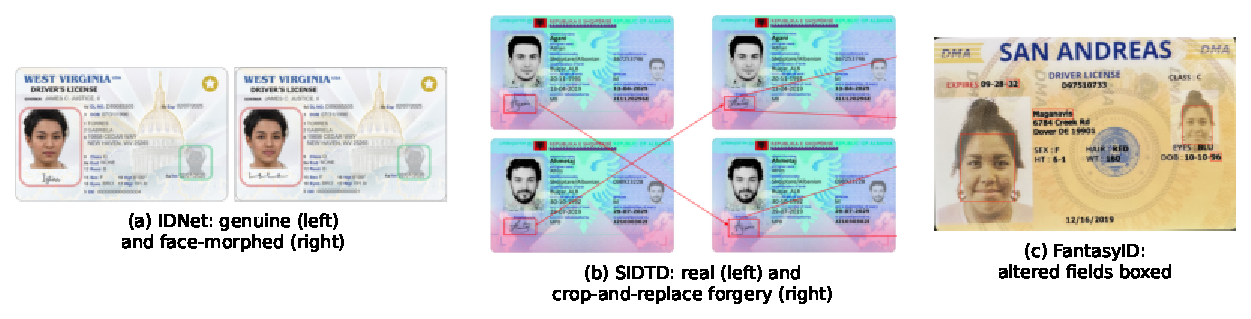
\includegraphics[width=\textwidth]{figures/fig_attacks.pdf}
\caption{What a digitally altered document looks like in the public datasets this study uses. (a) A genuine synthetic licence and its face-morphed version, with the ghost image also changed. (b) A real mock identity card and its crop-and-replace forgery, where the signature field has been moved and the background pattern is distorted. (c) A printed and photographed fantasy licence with the altered portrait, name, date of birth and expiry boxed. Panels reproduced from the IDNet \cite{guan2024idnet}, SIDTD \cite{boned2024sidtd} and FantasyID \cite{korshunov2025fantasyid} papers.}
\label{fig:attacks}
\end{figure}

\paragraph{Why the first-line decision is hard.} The alterations in Fig.~\ref{fig:attacks} leave no cue a human can see at counter speed. A morphed portrait matches both the bearer and the document. A replaced field keeps the font. A rewritten date keeps the guilloche. Chip verification catches a document whose chip signature fails, not one whose printed data page was altered behind a genuine or cloned chip. An examiner can learn 80 countries' security features over years of training; a first-line officer cannot, and a rare template is exactly where an officer either over-refers, feeding the 95.6 percent of clean referrals, or under-refers, which is the unmeasured miss.

\begin{keybox}
\noindent\textbf{Problem statement.} The first line decides refer or clear in seconds, across templates from more than 80 countries, with a commercial system whose behaviour on designs outside its library no vendor publishes and no operator can measure. Published detectors are no substitute: they memorize designs. This project builds the learned, reference-conditioned detector, measures it on public data against designs it has never seen, and reports the result in the centre's own terms, referrals and misses, so that GDRFA has both the number and the open instrument to obtain it on its own template library.
\end{keybox}

\begin{figure}[H]
\centering
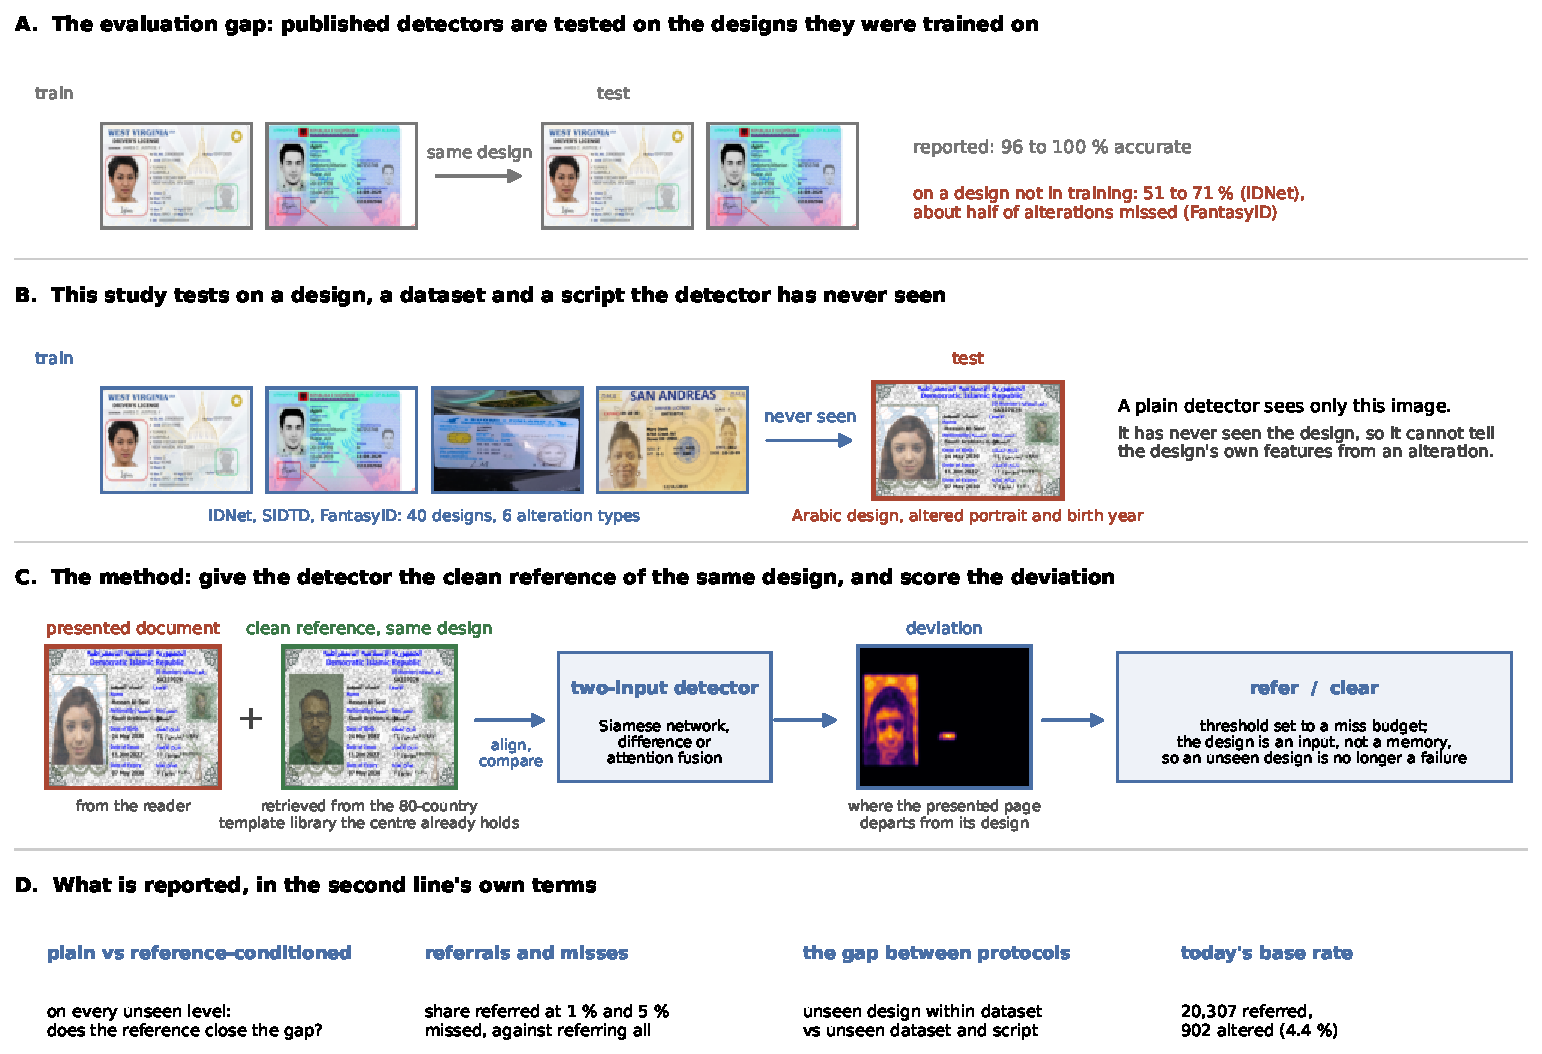
\includegraphics[width=\textwidth]{figures/fig_idea.pdf}
\caption{The idea. (A) Published detectors are evaluated on documents whose design was in training, where they score near 100 percent; on a new design the same detectors fall to chance. (B) This study trains on forty designs from three public datasets and tests on a design, a dataset and a script the detector has never seen; a plain detector has nothing to compare the page against. (C) The method gives the detector a second input, the clean reference of the same design, which at a border is the specimen in the template library, and scores the deviation between the two, here an altered portrait and birth year. (D) Results are reported as the gap the reference closes, the gap between the two protocols, referrals and misses, and the base rate. Document images from IDNet \cite{guan2024idnet}, SIDTD \cite{boned2024sidtd} and FantasyID \cite{korshunov2025fantasyid}; the presented document in (C) is a FantasyID card altered by us for illustration.}
\label{fig:idea}
\end{figure}

\paragraph{Contributions.} In the structure of our writer-identification study \cite{abushahla2026ijdar}, the contributions are:
\begin{enumerate}
\item \textbf{Data.} The first paired, design-referenced forgery dataset built from public sources: design medians and zone masks for 23 designs, annotated field layouts for FantasyID's 13 designs, about 5,000 forgeries with exact masks, and identity-grouped splits, released with the code.
\item \textbf{Benchmark.} The first evaluation of identity-document alteration detection under two protocols, unseen design within a dataset and unseen design across dataset, generator, capture and script, ending with an Arabic-script design, for single-image and reference-conditioned detectors on identical samples, with the gap between protocols quantified.
\item \textbf{Architecture.} A reference-conditioned detector built on a published change-detection framework, in a difference-fusion and an attention-fusion variant, with the modifications listed in Section~\ref{sec:arch}.
\item \textbf{Analysis.} A configuration grid over backbones, fusion, reference construction and transfer regime at three seeds, and the first referral-rate reading of a learned detector for first-line examination against a published base rate.
\end{enumerate}

\FloatBarrier
\section{Related work and the gap}
\label{sec:related}

\paragraph{Detectors memorize templates.} Learned forgery detectors for identity documents reach near-perfect accuracy when training and test documents share a design, and collapse when they do not. The IDNet authors report accuracy falling from 98.65 to 50.55 percent on face morphing and from 100 to 60.92 percent on text replacement when a detector trained on one US state's licence is tested on another's \cite{guan2024idnet}. The SIDTD authors added a nationality hold-out to their benchmark for this reason; their best backbones drop from 97 to 100 percent on seen nationalities to 82 to 91 percent on held-out ones, and their one two-image baseline, which pairs arbitrary documents, is the worst at 62.8 \cite{boned2024sidtd}. FantasyID's test split uses designs absent from training, and four published forensic detectors miss about half the manipulations at a 10 percent false-alarm point, with face swaps at an AUC of 56 to 62 \cite{korshunov2025fantasyid}. The 2025 DeepID challenge confirmed the pattern on 20,000 real documents: the winner scored an F1 of 0.99 on fantasy cards and 0.72 on real ones, every entry was near chance on single-field text edits with blending, and every system was a single-image forensics network of the TruFor family \cite{korshunov2025deepid,guillaro2023trufor}. Two 2026 surveys name this generalization failure as the central open problem of the field \cite{das2026survey,ruiz2025review}. The mechanism is that the learned cue, a noise residual, a compression trace, a font or a layout, is tied to the data-generating process and to the design, not to forgery; the DeepID winner's authors state that the decisive training cue was a JPEG quality difference between genuine and forged files \cite{korshunov2025deepid}.

\paragraph{Comparing against a reference is standard practice, but not as a learned detector.} Human examiners and commercial readers verify a document against a specimen of the same design. Regula's reader checks pattern shape, size, colour and position against a database of more than 13,000 templates, each authored by hand in about a working day \cite{regula2023templates}; PRADO and EdisonTD give examiners specimen images; and a vendor pipeline at the 2025 DeepID workshop matches structural similarity against a 128-country library \cite{idakto2025embedded}. These are closed, per-design rule sets with no published accuracy and no generalization beyond their templates. Learned two-input models for identity documents are rare and all on private data. CheckSim compares query patches with a reference model through a Siamese network on four French document types with per-type thresholds \cite{ghanmi2021checksim}. Chen et al.\ compare a questioned document with a reference of the same template to detect recapture rather than altered content, and the reference is what lets their detector transfer across document types \cite{chen2022domain}. Al-Ghadi et al.\ compare a query with a random genuine document of the same country and report true-accept rates above 0.92 on guilloche forgeries \cite{alghadi2022guilloche}; their follow-up removed the reference at test time and the published curves fell to an AUC near 0.5 \cite{alghadi2023fmidv}, a negative result that says the reference carried the generalization. The 2025 systematic review can cite one paper for the whole ``comparison with known references'' category \cite{ruiz2025review}. The one verified case of a template supplied at inference and evaluated on unseen document types on public data is for text recognition, not forgery: feeding the template through attention cut the error on unseen types from 0.81 to 0.31, while stacking it as an extra image channel did not work \cite{neitthoffer2023knowledge}. Outside documents the principle is mature: change detection subtracts Siamese features of two images \cite{daudt2018fcsiamdiff,fang2023changer}, and differential morphing attack detection at border gates compares the passport photo with a trusted live capture and reaches error rates that single-image detection cannot \cite{scherhag2020dmad}.

\paragraph{Nobody has framed the output as a referral.} ICAO Doc 9303 distinguishes inspection levels and states that machine-assisted authentication is to assist, not replace, the examiner \cite{icao9303p2}. The Schengen Handbook defines second-line checks \cite{eu2022handbook}. Frontex's Document Challenge exercises measured how well human officers and machines detect false documents at the first line and how to handle inconclusive results, with no learned detector \cite{gariup2019firstline}. Frontex counts 22,395 fraudulent documents detected at EU borders in 2023 \cite{frontex2023ara}. Yet no paper reports what a learned detector would do in those terms: the referral rate at a fixed miss budget, or the expert workload saved against a known base rate. The only methodological foothold is a 2026 benchmark finding that calibration, not representation, is the bottleneck of document forensics under domain shift \cite{docforge2026}.

\begin{keybox}
\noindent\textbf{The gap.} Detectors fail on unseen designs because a single image carries no model of what the design should look like. Examiners and commercial readers solve this by comparing against a specimen, and the two-input principle is established in change detection and differential morph detection, yet no learned identity-document alteration detector takes the clean reference of the same design as a second input and is evaluated on designs absent from training, on public data. The public benchmarks hold the ingredients: SIDTD has a nationality hold-out, FantasyID an unseen-design test split, and both have the field annotations from which a design reference can be built. No operator can get this number from its vendor. This proposal produces it.
\end{keybox}

\paragraph{Positioning.} Table~\ref{tab:position} places the proposal against the nearest prior work. The components are known: Siamese difference and attention fusion, registration against a specimen, a two-head output, a calibrated threshold. The contribution is putting the reference where the generalization failure is, building the public data to test it, and evaluating it the way the first line would use it.

\begin{table}[t]
\centering\small
\setlength{\tabcolsep}{4pt}
\caption{Positioning against the nearest prior work.}
\label{tab:position}
\begin{tabular}{L{3.3cm}L{1.8cm}L{2.0cm}L{2.3cm}L{1.5cm}L{1.8cm}}
\toprule
Work & Alteration type & Reference input & Unseen designs & Public data & Referral metric \\
\midrule
IDNet \cite{guan2024idnet} & digital & no & within dataset & yes & no \\
SIDTD \cite{boned2024sidtd} & digital & no (CoAARC pairs arbitrary images) & nationality hold-out & yes & no \\
FantasyID, DeepID \cite{korshunov2025fantasyid,korshunov2025deepid} & digital & no & unseen designs & partly & no \\
FakeIDet2 \cite{munozharo2026fakeidet2} & physical copy & no & cross-country & yes & no \\
CheckSim \cite{ghanmi2021checksim} & digital, patches & yes & no & no & no \\
Chen et al.\ \cite{chen2022domain} & recapture & yes & cross-type & no & no \\
Al-Ghadi et al.\ \cite{alghadi2022guilloche,alghadi2023fmidv} & guilloche copy-move & yes, then removed & no & yes & no \\
Neitthoffer et al.\ \cite{neitthoffer2023knowledge} & none (OCR) & yes, attention & leave-type-out & yes & no \\
Frontex exercises \cite{gariup2019firstline} & both & specimen, human & n/a & no & human \\
\textbf{This proposal} & digital & yes, learned, difference and attention & across datasets and scripts & yes, released & yes \\
\bottomrule
\end{tabular}
\end{table}

\FloatBarrier
\section{Objectives}
\label{sec:objectives}

\textbf{Aim.} Establish, on public data, whether conditioning a learned alteration detector on the clean reference of the presented design lets it generalize to document designs it has never seen, and report the result as a first-line referral decision.

\begin{enumerate}[label=\textbf{RQ\arabic*.}]
\item How much does a single-image detector lose when the test design, dataset or script was absent from training, and how much of that loss does the reference input recover, under each fusion?
\item How large is the gap between the two protocols, unseen design within a dataset and unseen design across dataset, generator, capture and script, and what drives it?
\item Which backbone, transfer regime and reference construction carry the gain, and is the attention-fusion variant worth its cost over difference fusion?
\item At a miss budget of 5 and 1 percent, what fraction of documents does the detector refer on designs it has never seen, compared with referring everything, which is today's second line?
\end{enumerate}

\FloatBarrier
\clearpage
\begin{landscape}
\begin{figure}[p]
\centering
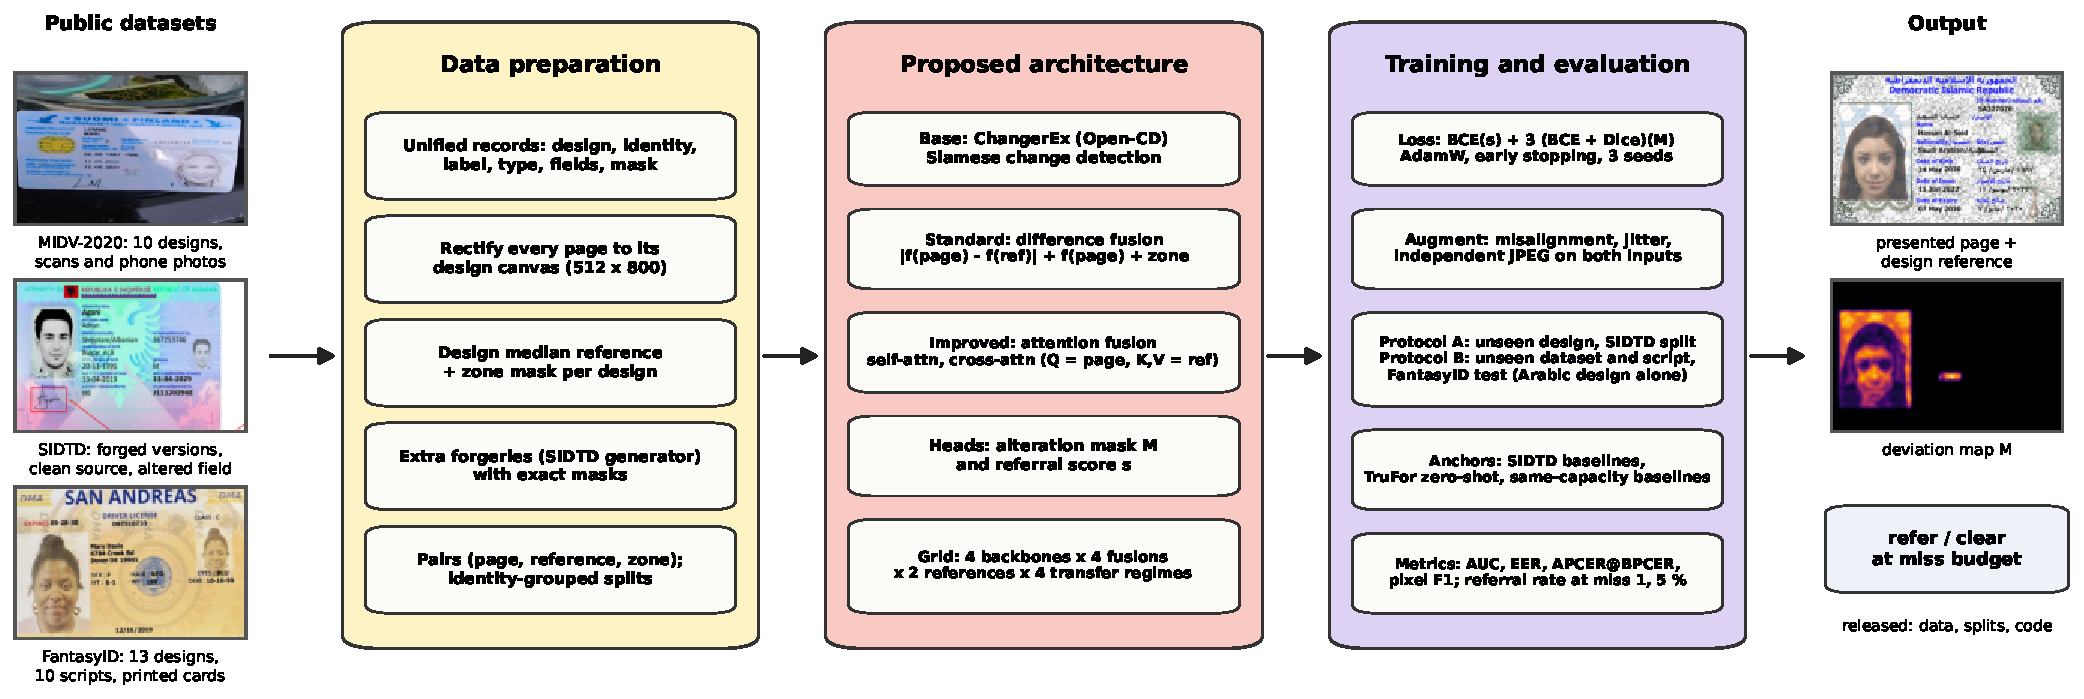
\includegraphics[width=\linewidth]{figures/fig_pipeline.pdf}
\caption{The project at a glance. Three public datasets are unified, rectified and paired with a design reference and a zone mask; a Siamese change-detection framework is extended into a standard (difference-fusion) and an improved (attention-fusion) reference-conditioned detector with a mask head and a referral head; both are trained on identical samples and evaluated under two protocols against the published baselines; the output is an alteration map and a refer-or-clear decision at a chosen miss budget. Data, splits and code are released.}
\label{fig:pipeline}
\end{figure}
\end{landscape}

\section{Methodology}
\label{sec:method}

\subsection{Overview and deployment}
\label{sec:overview}

\paragraph{Overview.} Figure~\ref{fig:pipeline} shows the project at a glance. Three public datasets are unified into one record format, every page is rectified onto its design canvas and paired with a reference of the same design and a zone mask (Section~\ref{sec:data}); a Siamese change-detection framework is extended into a standard and an improved reference-conditioned detector (Section~\ref{sec:arch}); both are trained on identical samples and evaluated under two protocols against the published baselines, and the score is turned into a referral decision (Section~\ref{sec:eval}); the configuration grid and the experiments are in Section~\ref{sec:exp}. Figure~\ref{fig:system} shows where the detector would sit at a counter.

\paragraph{Threat model.} The attacker presents a document whose data page has been digitally altered: a morphed or substituted portrait, an edited text field, an inpainted and rewritten region, or a combination. Physical copies and screen recaptures are a different task, presentation attack detection, and are out of scope. Attacks on the chip are out of scope; the chip path is unchanged. The attacker is assumed to know the genuine template well, which is why unseen-design evaluation matters: the detector must not depend on having seen the design.

\begin{figure}[htbp]
\centering
\resizebox{0.95\textwidth}{!}{%
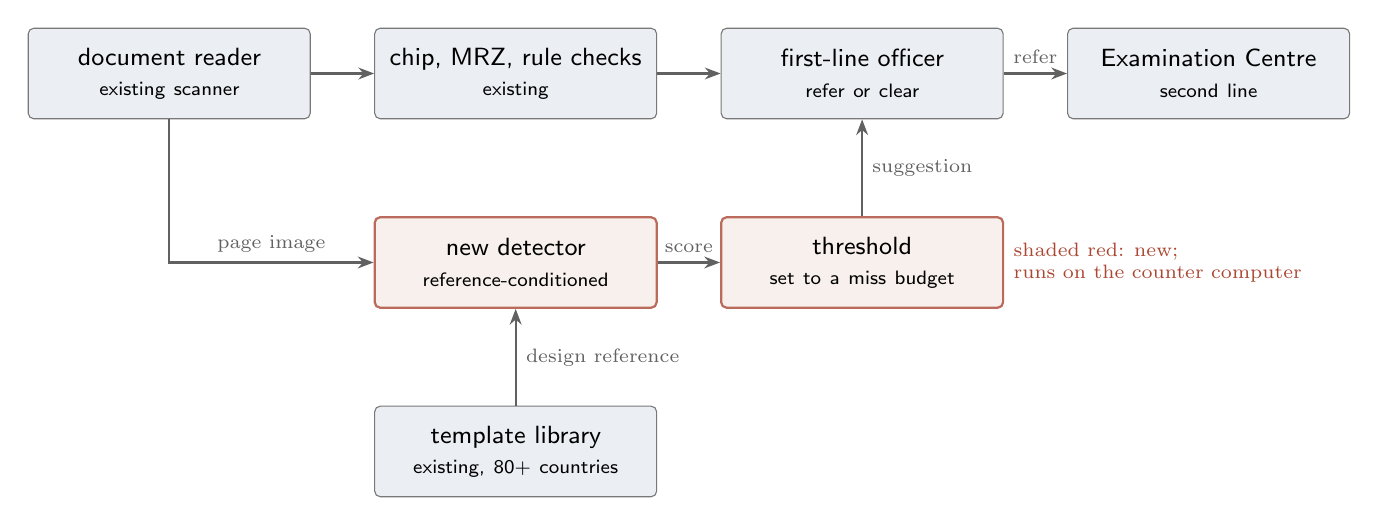
\begin{tikzpicture}[font=\sffamily\small, x=1cm, y=1cm,
  box/.style={draw=ink!60, fill=soft, rounded corners=2pt, align=center, minimum height=1.15cm, text width=3.3cm, inner sep=4pt},
  newb/.style={box, fill=soft2, draw=line2!80, thick},
  arr/.style={-{Stealth[length=2mm]}, thick, ink!70}]
\node[box] at (0,2.4) (read) {document reader\\ \scriptsize existing scanner};
\node[box] at (4.4,2.4) (chip) {chip, MRZ, rule checks\\ \scriptsize existing};
\node[box] at (8.8,2.4) (officer) {first-line officer\\ \scriptsize refer or clear};
\node[box] at (13.2,2.4) (centre) {Examination Centre\\ \scriptsize second line};
\node[newb] at (4.4,0) (det) {new detector\\ \scriptsize reference-conditioned};
\node[newb] at (8.8,0) (cal) {threshold\\ \scriptsize set to a miss budget};
\node[box] at (4.4,-2.4) (lib) {template library\\ \scriptsize existing, 80+ countries};
\draw[arr] (read) -- (chip);
\draw[arr] (chip) -- (officer);
\draw[arr] (officer) -- node[above, font=\scriptsize]{refer} (centre);
\draw[arr] (read.south) |- node[pos=0.75, above, font=\scriptsize]{page image} (det.west);
\draw[arr] (lib) -- node[right, font=\scriptsize]{design reference} (det);
\draw[arr] (det) -- node[above, font=\scriptsize]{score} (cal);
\draw[arr] (cal) -- node[right, font=\scriptsize]{suggestion} (officer);
\node[font=\scriptsize, text=line2, align=left, anchor=west] at (10.6,0) {shaded red: new;\\ runs on the counter computer};
\end{tikzpicture}}
\caption{Where the detector sits. The reader already captures the data page and the centre already holds the template library; the detector receives both on the counter computer, scores the deviation, and a threshold set to the miss budget turns the score into a referral suggestion beside the existing checks. The officer still decides, as ICAO Doc 9303 requires, and the second line is unchanged.}
\label{fig:system}
\end{figure}

\FloatBarrier
\subsection{Data and preparation}
\label{sec:data}

\paragraph{Datasets.} All sets are public, openly licensed, and downloadable without a request form (Table~\ref{tab:data}); figure~\ref{fig:templates} shows the template diversity. MIDV-2020 provides ten real document designs, one hundred mock identities each, rendered templates and their printed, scanned and phone-photographed captures, with a rectangle and value for every field. SIDTD provides forged versions of those documents, each naming its clean source and the field it altered, together with the published nationality hold-out split and the code that produced the forgeries. FantasyID provides thirteen fictional designs in ten scripts, among them Arabic, printed on PVC cards and photographed on two phones and a scanner, with face swaps and text edits from generators different from SIDTD's, and an official test split whose designs are absent from training. No real traveller's document appears anywhere.

\begin{table}[htbp]
\centering\small
\setlength{\tabcolsep}{4pt}
\caption{Public datasets used. All licences permit research use and release of derived data.}
\label{tab:data}
\begin{tabular}{L{2.1cm}L{3.6cm}L{3.0cm}L{2.0cm}L{2.6cm}}
\toprule
Dataset & Content & Alteration classes & Licence & Role \\
\midrule
MIDV-2020 \cite{bulatov2022midv2020} & 10 designs $\times$ 100 identities; templates, scans, phone photos; every field rectangle & none (genuine) & CC BY-SA 2.5 & genuine class; design medians; zone masks; capture variation \\
SIDTD \cite{boned2024sidtd} & 1,222 forged versions of the MIDV-2020 templates, each with its clean source and altered field; nationality hold-out split; generator code & crop-and-replace, inpaint-and-rewrite & CC BY-SA & altered class; Protocol A split; extra forgeries with exact masks \\
FantasyID \cite{korshunov2025fantasyid} & 13 printed fantasy designs, 10 scripts incl.\ Arabic, 1,086 bona fide captures on 3 devices; official test split with 3 designs absent from training & face swap (2 generators), text inpainting (2 generators) & CC BY 4.0 & Protocol B test, never trained on \\
IDNet \cite{guan2024idnet}, optional & 837,060 synthetic documents, 20 designs & morph, portrait swap, text edit, inpaint, crop-move & CC0 / CC BY 4.0 & volume experiment only \\
\bottomrule
\end{tabular}
\end{table}

\begin{figure}[htbp]
\centering
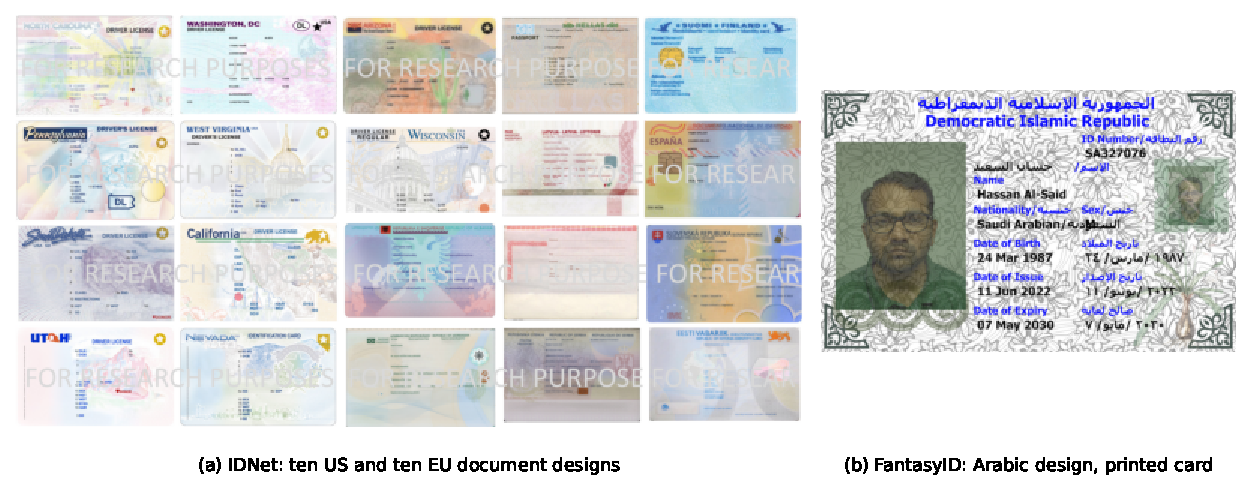
\includegraphics[width=\textwidth]{figures/fig_templates.pdf}
\caption{Template diversity in the public sets. (a) The twenty designs IDNet is generated from, watermarked by its authors. (b) One of FantasyID's thirteen designs, in Arabic script, after printing on a PVC card and photographing; this design is reported on its own as the Dubai case. Reproduced from \cite{guan2024idnet} and \cite{korshunov2025fantasyid}.}
\label{fig:templates}
\end{figure}

\paragraph{The reference and the zone mask.} The detector takes two inputs, the presented data page $x$ and a reference $r$ of the same design (Fig.~\ref{fig:idea}C), plus a zone mask $z$ marking the personal-data fields. The reference must be what an officer could have: the design, not the person. Using the same person's clean document would reduce the task to a pixel difference and does not exist at a border. We therefore build, for every design, a \emph{design median}: the pixel-wise median over all genuine documents of that design after rectification, in which personal content varies across identities and is removed while the static design, guilloche, headings, field labels and borders, survives. At Dubai's border the reference is the specimen in the centre's own library \cite{gulfnews2026forgery}. The zone mask tells the network where content is expected to differ: inside personal fields it must find inconsistency with the design, a font, a baseline, a colour, a guilloche discontinuity at the field edge, while outside them any difference is suspicious.

\paragraph{Registration and the wrong reference.} Every page is identified and rectified onto its design canvas at $512 \times 800$, using the annotated document quadrilateral where the dataset provides one and otherwise feature matching against the design medians with a robust homography, which is the standard first step of commercial readers and of the MIDV authors' pipeline \cite{bulatov2022midv2020}, followed by a local refinement. The residual registration error is kept and reported. A page that matches no design closely enough returns ``unknown design'', which at the border means refer; the network is also trained with wrong-design pairs labelled altered so that it fails safe.

\paragraph{Records, pairs and splits.} One record per image: design, identity, binary label, alteration type, capture device, field rectangles, and the altered-region mask. Field rectangles are native for MIDV-2020 and SIDTD and annotated once by us for FantasyID's thirteen layouts. Altered-region masks come from the recorded field rectangle in SIDTD, and, where we rerun SIDTD's released generator on the MIDV-2020 templates to raise the altered class from 1,222 to about 5,000 documents, from the generator itself, so that those masks are exact. Samples are paired as (page, reference, zone mask); genuine pages are paired with a reference built without their own identity; wrong-design pairs are added as hard negatives. Splits are grouped by identity, and FantasyID's three captures of a card stay together. The paired dataset, the layouts, the medians and the splits are released.

\FloatBarrier
\subsection{Proposed architecture}
\label{sec:arch}

\paragraph{Base framework.} The base framework is ChangerEx \cite{fang2023changer}, a Siamese change-detection network in the Open-CD toolbox \cite{li2025opencd}, chosen because it compares the two streams inside the backbone through feature exchange and because its flow-alignment fusion tolerates the residual misregistration a photographed card always has; pretrained change-detection checkpoints exist. Two variants, sharing every tensor size, play the roles of the standard and attention-based architectures of our writer-identification study \cite{abushahla2026ijdar}.

\begin{itemize}
\item \textbf{Standard variant, difference fusion.} A shared encoder processes the page $x$ and the reference $r$. At each scale the absolute feature difference $|f(x) - f(r)|$ is concatenated with $f(x)$, because alteration artifacts are one-sided and live only in the page, and with the downsampled zone mask. The decoder emits the alteration mask $M$; a new global head, global average pooling of the deepest fused features concatenated with $\max M$ and two dense layers, emits the score $s$.
\item \textbf{Improved variant, attention fusion.} Three attention blocks inserted without changing tensor sizes: self-attention over the page's deepest features, so that a replaced field and its surroundings attend to each other; cross-attention in which the page features are the queries and the reference features the keys and values, so that each location reads what the design should contain there, the learned form of comparing against the specimen and the fusion the unseen-ID-type study found necessary where channel stacking failed \cite{neitthoffer2023knowledge}; and cross-attention from the pooled global descriptor over the fused local features before the score head. The zone mask enters as a bias on the cross-attention logits. Six heads, key dimension 32.
\end{itemize}

The named modifications to the base framework are therefore: zone-conditioned fusion, one-sided page concatenation, cross-attention reference fusion, the global referral head, the joint loss over score and mask, the design-median reference construction, and wrong-design training pairs. Figure~\ref{fig:arch} draws both variants.

\begin{figure}[H]
\centering
\resizebox{\textwidth}{!}{%
\begin{tikzpicture}[font=\sffamily\scriptsize, x=1cm, y=1cm,
  blk/.style={draw=ink!70, rounded corners=2pt, align=center, minimum height=0.95cm, text width=2.15cm, inner sep=3pt, fill=soft},
  attn/.style={blk, fill=soft2, draw=line2!80, dashed, thick},
  outb/.style={blk, fill=white, draw=line1!80, thick, text width=1.8cm},
  lab/.style={font=\sffamily\scriptsize, align=center},
  arr/.style={-{Stealth[length=1.8mm]}, thick, ink!70},
  darr/.style={arr, dashed, line2!80}]
% inputs
\node[inner sep=0, draw=line2!80, thick] at (0,2.4) (x) {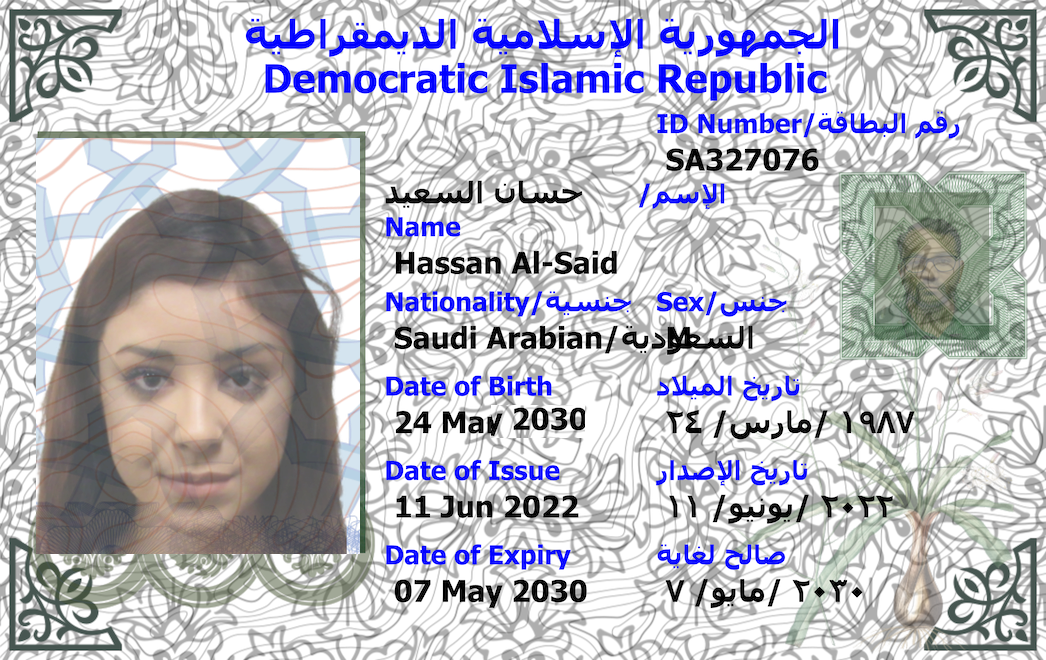
\includegraphics[width=1.7cm]{figures/arch_presented.png}};
\node[lab, below=1pt of x] {page $x$};
\node[inner sep=0, draw=ink!60] at (0,0.6) (r) {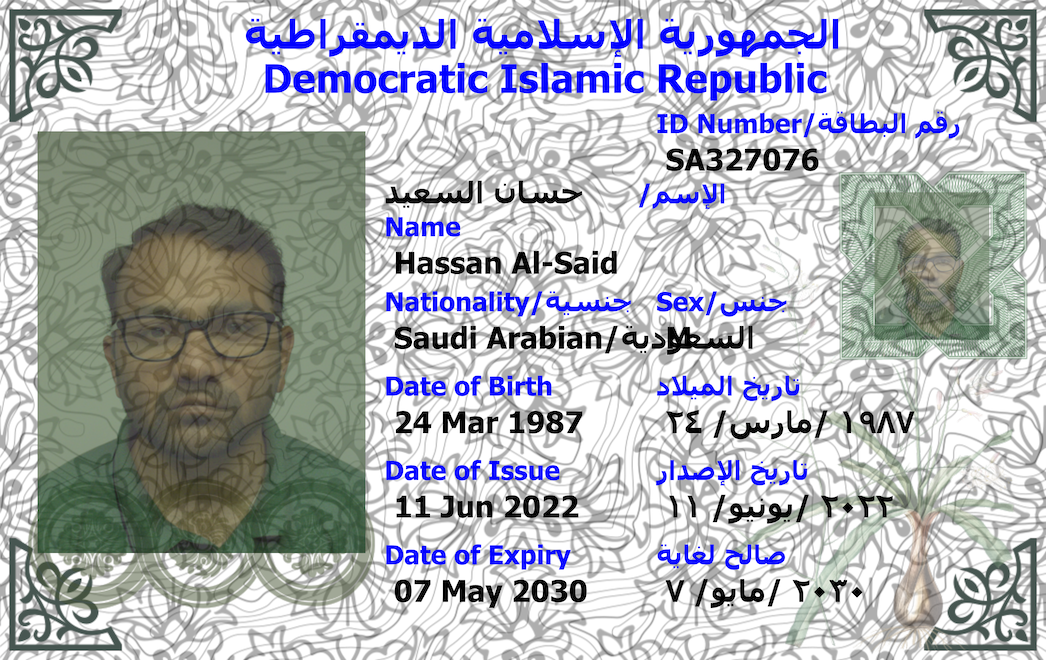
\includegraphics[width=1.7cm]{figures/arch_reference.png}};
\node[lab, below=1pt of r] {design reference $r$};
\node[inner sep=0, draw=ink!60] at (0,-1.2) (z) {
\includegraphics[width=1.7cm]{figures/arch_zone.png}};
\node[lab, below=1pt of z] {zone mask $z$};
% encoders
\node[blk] at (2.8,2.4) (ex) {encoder\\ \scriptsize ResNet / ResNeSt / MiT};
\node[blk] at (2.8,0.6) (er) {encoder\\ \scriptsize same weights};
\draw[<->, dotted, thick, ink!60] (ex.south) -- node[right, font=\scriptsize]{shared} (er.north);
% exchange
\node[blk, minimum height=2.75cm] at (5.6,1.5) (fx) {feature exchange\\ and flow alignment\\ \scriptsize (ChangerEx)};
% middle row
\node[blk] at (8.4,1.5) (diff) {difference fusion\\ \scriptsize $|f(x)-f(r)| \oplus f(x) \oplus z$};
\node[blk] at (11.2,1.5) (dec) {decoder\\ \scriptsize (ChangerEx)};
\node[outb] at (14.0,1.5) (m) {alteration mask $M$};
\node[inner sep=0, draw=line1!80, thick] at (16.3,1.5) (mi) {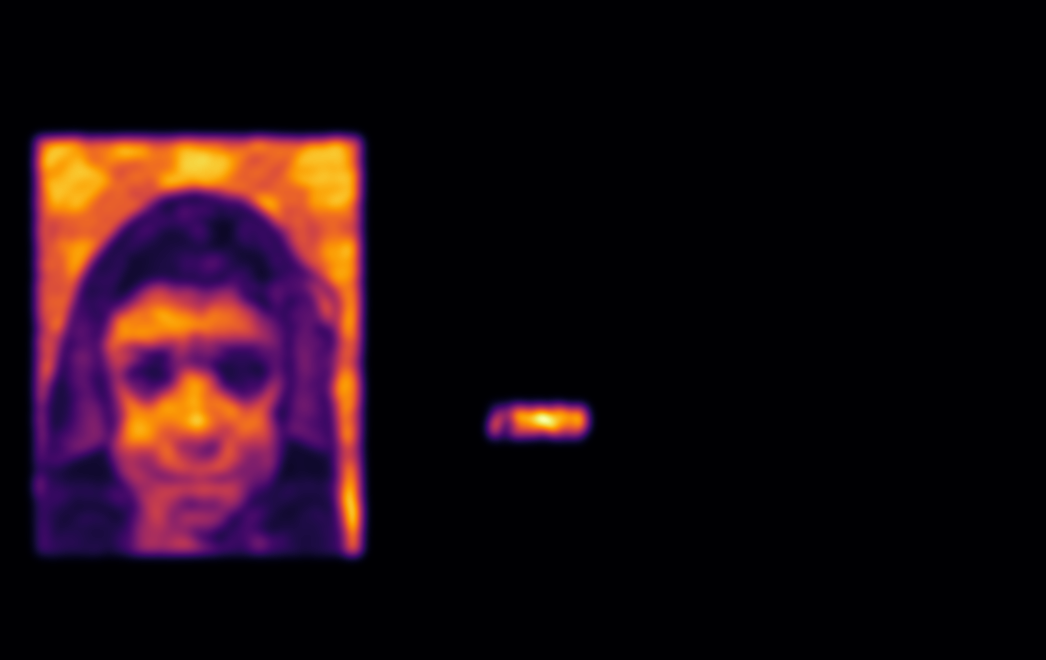
\includegraphics[width=1.7cm]{figures/arch_mask.png}};
% top row: improved variant
\node[attn] at (8.4,3.7) (sa) {self-attention\\ \scriptsize over $f(x)$};
\node[attn] at (11.2,3.7) (ca) {cross-attention\\ \scriptsize $Q{=}f(x)$, $K{=}V{=}f(r)$};
% bottom row: score head
\node[blk] at (11.2,-0.9) (gap) {global pooling\\ \scriptsize GAP $\oplus$ $\max M$};
\node[attn] at (14.0,-0.9) (ca2) {cross-attention\\ \scriptsize global over local};
\node[outb] at (16.3,-0.9) (sc) {score $s$\\ \scriptsize refer / clear};
% arrows, standard path
\draw[arr] (x) -- (ex); \draw[arr] (r) -- (er);
\draw[arr] (ex.east) -- (ex.east -| fx.west);
\draw[arr] (er.east) -- (er.east -| fx.west);
\draw[arr] (fx) -- (diff);
\draw[arr] (z.east) -- (z.east -| diff.south) -- (diff.south);
\draw[arr] (diff) -- (dec);
\draw[arr] (dec) -- (m);
\draw[arr] (m) -- (mi);
\draw[arr] (dec.south) -- (gap.north);
\draw[arr] (m.south) -- ++(0,-0.55) -| ($(gap.north)+(0.7,0)$);
\node[font=\scriptsize, anchor=south] at (13.1,0.5) {$\max M$};
\draw[arr] (gap.south) -- ++(0,-0.5) -| (sc.south);
\node[font=\scriptsize, text=ink!60, anchor=north] at (13.75,-1.9) {standard: pooled features to score};
% arrows, improved path
\draw[darr] (fx.north) |- (sa.west);
\draw[darr] (sa) -- (ca);
\draw[darr] (ca) -- (dec);
\draw[darr] (gap) -- (ca2);
\draw[darr] (ca2) -- (sc);
\node[font=\scriptsize, text=line2, align=left, anchor=west] at (12.6,3.7) {dashed: improved\\ variant only};
\end{tikzpicture}}
\caption{Proposed architecture. Solid blocks and arrows form the standard variant: the page and the design reference pass through one shared encoder, ChangerEx exchanges and aligns their features, the absolute difference is concatenated with the page features and the zone mask, and a decoder emits the alteration mask while a global head emits the referral score. Dashed blocks form the improved variant: self-attention over the page features, cross-attention in which the page queries the reference with the zone mask as a bias, and a final cross-attention from the global descriptor over the fused local features. Tensor sizes are identical in both variants.}
\label{fig:arch}
\end{figure}

\paragraph{Input, output, training.} Input: the page, the reference and the zone mask on the $512 \times 800$ design canvas. Output: an alteration mask and one score; the decision is binary, genuine or altered, and alteration type is reported per class, not predicted. Loss: binary cross-entropy on the score plus three times binary cross-entropy and Dice on the mask. AdamW with a cosine schedule, batch 8, 40 epochs, mixed precision, a learning-rate scheduler and early stopping on identity-disjoint validation AUC, three seeds with mean and standard deviation. Augmentation: random affine of up to 8 pixels between the two inputs, photometric jitter, and independent JPEG recompression at quality 60 to 100 on each input so that compression cannot become the cue.

\FloatBarrier
\subsection{Evaluation}
\label{sec:eval}

\paragraph{Protocols.} Two protocols, in the manner of the line-level and page-disjoint protocols of our writer-identification study \cite{abushahla2026ijdar}, so that the gap between them is itself a result (Fig.~\ref{fig:protocol}).

\begin{itemize}
\item \textbf{Protocol A, unseen design within a dataset.} Train on six MIDV nationalities, test on the other four, using SIDTD's published split file, so that our numbers sit beside the SIDTD authors' own baselines on the same images: EfficientNet-B3 at 82.0 percent accuracy and AUC 0.899, ResNet50 at 90.6 and 0.963, ViT-L at 91.0 and 0.969, and the two-image CoAARC at 62.8 and 0.675 \cite{boned2024sidtd}.
\item \textbf{Protocol B, unseen dataset, generator, capture and script.} Train on all ten MIDV designs, test on FantasyID's official test split of 300 genuine and 1,085 altered cards, never having seen FantasyID. The published FantasyID baselines are pretrained forensic detectors that likewise never saw it, so the comparison is like for like: TruFor at AUC 93.5 overall and 55.8 on face swaps, MMFusion at HTER 25.8, UniFD and FatFormer at chance \cite{korshunov2025fantasyid}. We run TruFor's public weights ourselves to validate the pipeline against its printed numbers \cite{guillaro2023trufor}. The Arabic design is reported separately, with zero and ten calibration cards, as the Dubai case; no published number exists for it.
\end{itemize}

\begin{figure}[H]
\centering
\resizebox{0.85\textwidth}{!}{%
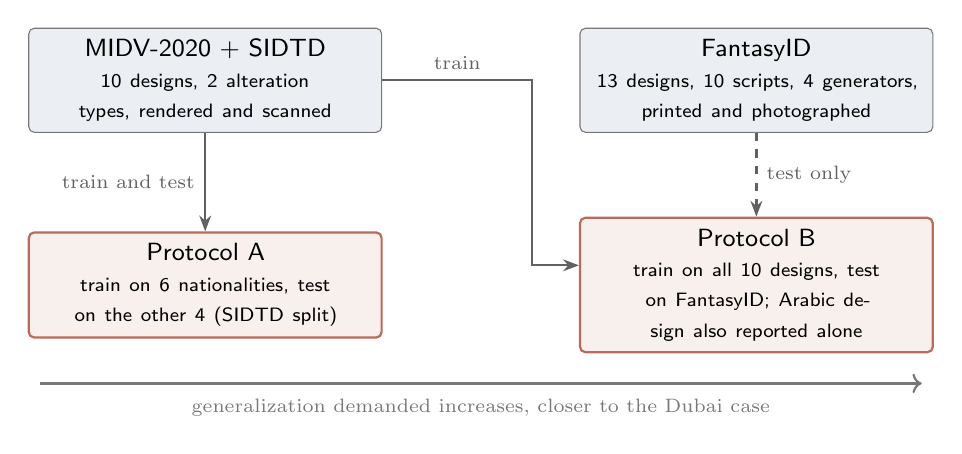
\begin{tikzpicture}[font=\sffamily\small, x=1cm, y=1cm,
  ds/.style={draw=ink!60, fill=soft, rounded corners=2pt, align=center, minimum height=1.3cm, text width=4.2cm, inner sep=4pt},
  tst/.style={ds, fill=soft2, draw=line2!80, thick},
  arr/.style={-{Stealth[length=2mm]}, thick, ink!70}]
\node[ds] at (0,2.6) (a) {MIDV-2020 + SIDTD\\ \scriptsize 10 designs, 2 alteration types, rendered and scanned};
\node[ds] at (7,2.6) (c) {FantasyID\\ \scriptsize 13 designs, 10 scripts, 4 generators, printed and photographed};
\node[tst] at (0,0) (l1) {Protocol A\\ \scriptsize train on 6 nationalities, test on the other 4 (SIDTD split)};
\node[tst] at (7,0) (l2) {Protocol B\\ \scriptsize train on all 10 designs, test on FantasyID; Arabic design also reported alone};
\draw[arr] (a) -- node[left, font=\scriptsize]{train and test} (l1);
\draw[arr] (a.east) -- node[above, font=\scriptsize]{train} ($(c.west)+(-0.6,0)$) |- ($(l2.west)+(0,0.25)$);
\draw[arr, dashed] (c) -- node[right, font=\scriptsize]{test only} (l2);
\draw[->, thick, ink!60] (-2.1,-1.25) -- (9.1,-1.25) node[pos=0.5, below=2pt, font=\scriptsize]{generalization demanded increases, closer to the Dubai case};
\end{tikzpicture}}
\caption{The two protocols. Solid arrows are training sources; the dashed arrow marks a test-only set. The same detectors, trained on identical samples, are evaluated under both, and the gap between the protocols is reported as a result.}
\label{fig:protocol}
\end{figure}

Table~\ref{tab:compare} lists, for each protocol, what our detectors are compared against and on which metric. Every row includes our two same-capacity baselines, the single-image and the channel-stacked network trained on identical samples, so that the effect of the reference is measured inside the study as well as against the literature.

\afterpage{%
\begin{landscape}
\begin{table}[p]
\centering\small
\setlength{\tabcolsep}{5pt}
\renewcommand{\arraystretch}{1.15}
\caption{What each protocol is compared against. Published numbers are copied from the cited papers on the same test data; ``ours'' are run in this study on identical samples.}
\label{tab:compare}
\begin{tabular}{L{2.9cm}L{3.9cm}L{8.2cm}L{3.2cm}L{3.5cm}}
\toprule
Protocol (experiment) & Train / test & Published baselines on the same test data & Our baselines & Compared on \\
\midrule
A, unseen design within dataset (E1) & SIDTD/MIDV, 6 nationalities / other 4, SIDTD split file & SIDTD paper \cite{boned2024sidtd}: EfficientNet-B3 82.0\,\% / 0.899; ResNet50 90.6\,\% / 0.963; ViT-L/16 91.0\,\% / 0.969; TransFG 83.6\,\% / 0.907; CoAARC (two images) 62.8\,\% / 0.675 & single-image and channel-stacked, four backbones & accuracy and AUC as published; plus EER, APCER at BPCER 1 and 5\,\% \\
\addlinespace
B, unseen dataset, generator, capture, script (E2) & all 10 MIDV designs / FantasyID official test, 300 genuine, 1,085 altered & FantasyID paper \cite{korshunov2025fantasyid}, all zero-shot: TruFor AUC 93.5 (text 99.5, face 55.8), HTER 33.4; MMFusion AUC 94.4 (face 61.5), HTER 25.8; UniFD AUC 52.0, HTER 50.5; FatFormer AUC 53.5, HTER 49.4. TruFor re-run by us from public weights \cite{guillaro2023trufor} & single-image and channel-stacked, four backbones & AUC and HTER as published, per alteration type; FNR at 10\,\% FPR \\
\addlinespace
B, Arabic design alone (E3) & as B / FantasyID Arabic design only, 0 and 10 calibration cards & none published; TruFor re-run as the external reference & single-image and channel-stacked & AUC, EER, APCER at BPCER 5\,\% \\
\addlinespace
Fine-tuned, optional (E8) & FantasyID train / FantasyID test & DeepID 2025, FantasyID part of the leaderboard \cite{korshunov2025deepid}, F1 at 0.5: Sunlight 0.991, EdgeDoc 0.958, Incode 0.868, TruFor 0.807, TruForID 0.712; the private real-ID half is not public & single-image & F1 at threshold 0.5 \\
\addlinespace
All protocols (E7) & as above & none: no paper reports a referral rate & single-image and channel-stacked & referral rate at miss 1 and 5\,\%; prior 4.4\,\% \\
\bottomrule
\end{tabular}
\end{table}
\end{landscape}}

\paragraph{Metrics.} Image level: AUC, equal error rate, attack presentation classification error rate at bona fide error rates of 1 and 5 percent, and half total error rate, the ISO/IEC 30107-3 vocabulary that the FantasyID and DeepID papers use; accuracy where the SIDTD baselines report it \cite{iso30107}. Mask level: pixel F1 and intersection over union. Operator level: referral rate at miss rates of 1 and 5 percent, with the centre's 4.4 percent as the prior.

\noindent\begin{minipage}[t]{0.55\textwidth}
\vspace{0pt}
\setlength{\parskip}{0.35em}
\textbf{The referral decision.} The detector outputs a score $s$. Let $p$ be the prior probability that a presented document is altered and $t$ a threshold. The first line refers when $s > t$. The two quantities GDRFA can act on are the referral rate $R(t) = (1-p)\,P(s > t \mid \text{genuine}) + p\,P(s > t \mid \text{altered})$ and the miss rate $M(t) = P(s \le t \mid \text{altered})$. We report $R$ at $M \in \{1\%, 5\%\}$, with $t$ chosen on a calibration split that contains no test design. Figure~\ref{fig:referral} shows what the trade-off looks like; the quantity of interest is where the measured curves lie on designs the detector has never seen.
\end{minipage}\hfill
\begin{minipage}[t]{0.42\textwidth}
\vspace{0pt}
\centering
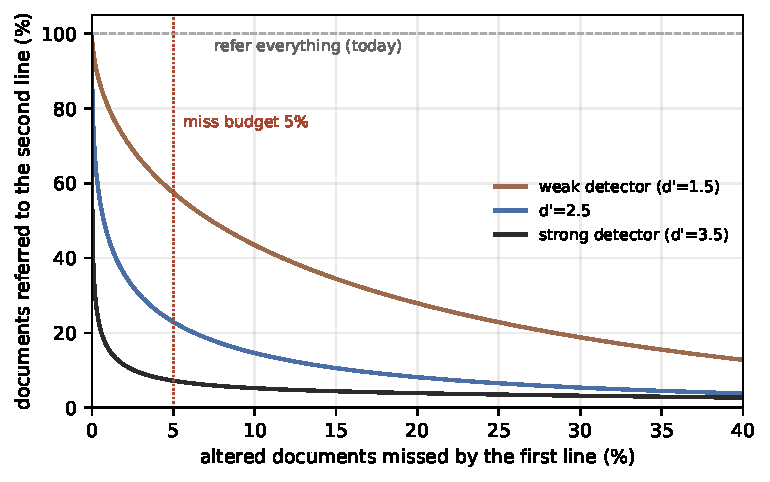
\includegraphics[width=\linewidth]{figures/fig_referral.pdf}
\captionof{figure}{The referral trade-off, sketched with a Gaussian score model at three separabilities; not a result. The dashed line is today's practice, refer everything.}
\label{fig:referral}
\end{minipage}

\FloatBarrier
\subsection{Configuration grid and experiments}
\label{sec:exp}

\paragraph{Configuration grid and baselines.} Four interchangeable backbones (ResNet-18, ResNet-50, ResNeSt-50, MiT-B1), four fusion settings (single-image with the same encoder and heads, channel-stacked early fusion, difference fusion, attention fusion), two reference constructions (design median, masked exemplar), and four transfer regimes (frozen backbone, partial and full fine-tuning, from scratch; change-detection against ImageNet initialization), three seeds each. The main table is the four backbones by the four fusion settings under both protocols; the single-image and channel-stacked settings are the same-capacity baselines, and the published SIDTD and FantasyID numbers above are the external anchors. Table~\ref{tab:experiments} maps the experiments to the research questions.

\begin{table}[H]
\centering\footnotesize
\setlength{\tabcolsep}{4pt}
\caption{Experiments. All report the image-level, mask-level and referral metrics, per alteration type.}
\label{tab:experiments}
\begin{tabular}{L{1.1cm}L{7.2cm}L{5.6cm}}
\toprule
RQ & Experiment & What it establishes \\
\midrule
RQ1 & E1, Protocol A: 4 backbones $\times$ 4 fusion settings, SIDTD nationality hold-out & loss on an unseen design and how much each fusion recovers \\
RQ1, RQ2 & E2, Protocol B: the same grid, trained on all 10 designs, tested on FantasyID; TruFor alongside & transfer across dataset, generator, capture and script; the gap between protocols \\
RQ1 & E3, the Arabic design with 0 and 10 calibration cards & the Dubai case and its calibration cost \\
RQ3 & E4, transfer regimes; E5, reference construction, zone mask, fusion and attention-bias ablations & which part of the method carries the gain \\
RQ3 & E6, wrong-design reference with and without the gate; misregistration sweep 0 to 12 px & failure modes and the fail-safe \\
RQ4 & E7, referral curves on all protocols; referral rate at miss 1 and 5\,\% & the operator metric \\
opt. & E8, fine-tune on FantasyID train, F1 at 0.5; E9, IDNet added to Protocol B training & the DeepID-comparable column; the volume effect \\
\bottomrule
\end{tabular}
\end{table}

\FloatBarrier
\section{Work plan, risks, relevance}
\label{sec:plan}

\begin{figure}[h]
\centering
\resizebox{\textwidth}{!}{\begin{ganttchart}[hgrid,vgrid,x unit=0.95cm,y unit chart=0.5cm,y unit title=0.55cm,
  title label font=\sffamily\scriptsize, bar label font=\sffamily\scriptsize, bar/.append style={fill=line1!35, draw=line1!70},
  milestone/.append style={fill=line2, draw=line2}, milestone label font=\sffamily\scriptsize]{1}{8}
\gantttitle{Days from start, 8 to 15 October 2026}{8}\\
\gantttitlelist{1,...,8}{1}\\
\ganttbar{download MIDV-2020, SIDTD, FantasyID; loader; design medians}{1}{1}\\
\ganttbar{rectification, FantasyID layouts, extra forgeries, splits}{2}{2}\\
\ganttbar{both variants in Open-CD; Protocol A grid (E1)}{3}{3}\\
\ganttbar{Protocol B grid, Arabic design, TruFor anchor (E2, E3)}{4}{4}\\
\ganttbar{ablations, robustness, referral curves (E4 to E7)}{5}{5}\\
\ganttbar{optional E8, E9; reruns; figures from real outputs}{6}{6}\\
\ganttbar{write, internal review}{6}{8}\\
\ganttmilestone{submit}{8}
\end{ganttchart}}
\caption{Eight-day plan to the 15 October deadline. The three core sets total about 10 GB; the grid runs as a cluster job array.}
\label{fig:gantt}
\end{figure}

\paragraph{Risks.} The reference may not help enough: the one prior two-image SIDTD baseline, which pairs arbitrary documents, was the worst performer on unseen nationalities, and Al-Ghadi's with-reference results were on an easy task. The design median, the zone mask and the attention fusion are exactly what those attempts lacked, and the ablations isolate them; a clear positive under Protocol A with a weaker result under Protocol B is still a publishable finding under the referral framing. The public forgeries are composites and generative edits, not professional counterfeits, the reality gap named by the surveys \cite{das2026survey,ruiz2025review}; the paper states that a leave-design-out number measures robustness to design change, not to a skilled forger, and treats the DeepID fantasy-to-real drop as the calibration a reader should apply. Registration on phone photos may fail on some cards; the failure rate is reported and failures count as referrals. The 4.4 percent base rate is among referrals, not travellers, and is used only to set the axis of the referral chart. The grid is about 300 GPU-hours and runs as a cluster array; if compute is short it is cut to two backbones.

\paragraph{Relevance to the award.} The work sits in the Digital Innovation Award, under artificial intelligence and data analytics \cite{gdrfa2026award}. It answers a challenge the Document Examination Centre has described in its own words, in the metric the centre publishes, and it gives the operator what its vendor does not: a measured answer to how a reference-based detector behaves on a design outside the library, together with the open dataset, protocol and model to repeat that measurement on GDRFA's own template library, on the counter computer it already has, with no document leaving the centre. A new design is then handled by adding its specimen, not by authoring rules or retraining.

\paragraph{Ethics and data.} No real identity document is used. MIDV-2020 and SIDTD use mock documents built from public-domain specimen images with generated faces and consenting volunteers, and FantasyID's faces are from consented or licensed sources with fictional designs. All licences permit the use and the release of derived data under the same terms.

\bibliographystyle{IEEEtran}
\bibliography{references}

\end{document}
